\documentclass{article}
\usepackage[most]{tcolorbox}
\usepackage{array}
\usepackage[table,dvipsnames]{xcolor}
\usepackage{graphicx, float}
\usepackage[T1]{fontenc}
\usepackage[utf8]{inputenc}
\usepackage[sfdefault]{atkinson}
\graphicspath{{images/}}
\usepackage{amsthm, amssymb, amsmath}
\usepackage[a4paper]{geometry}
\usepackage[skip=8pt, indent=0pt]{parskip}
\usepackage{pgfplots}
\usepackage[hidelinks]{hyperref}
\usepackage{cancel}
\pgfplotsset{width=8cm,compat=1.9}
\geometry{
a4paper,
total={170mm,257mm},
left=20mm,
top=20mm,
}

\DeclareUnicodeCharacter{221E}{\ensuremath{\infty}}

\title{Algoritmi}
\author{Marco Pittarello}
\date{}

\newtcbtheorem{theo}{Teorema}{
    colframe=BrickRed!100!white,
    colback=red!5!white
}{th}

\newtcbtheorem{ex}{Esempio}{
    colframe=OliveGreen!100!white,
    colback=OliveGreen!5!white
}{ex}

\newtcbtheorem{defi}{Definizione}{
    colframe=blue!100!white,
    colback=blue!10!white
}{def}

\newtcbtheorem{info}{Info}{
    colframe=cyan!80!black,
    colback=cyan!5!white
}{inf}

\newtcbtheorem{warn}{Attenzione}{
    colframe=orange!90!black,
    colback=orange!5!white
}{wrn}

\newtcbtheorem{tip}{Suggerimento}{
    colframe=purple!80!black,
    colback=purple!5!white
}{tip}

\newtcbtheorem{note}{Nota}{
    colframe=gray!80!black,
    colback=gray!5!white
}{nt}

\renewcommand{\arraystretch}{2}
\setlength{\tabcolsep}{20pt}

\begin{document}
\maketitle
\tableofcontents
\newpage

%-----------------------------------------------------------------------
\begin{defi}{Algoritmo}{}
Procedura che con semplici istruzioni descrive come risolvere un problema.
\end{defi}

Di ogni algoritmo bisogna sapere:
\begin{itemize}
    \item Correttezza
    \item Stabilità
    \item Complessità
\end{itemize}

%-----------------------------------------------------------------------
\section{Insertion Sort}

\begin{info}{Idea}{}
Si costruisce incrementalmente un sottoarray ordinato \texttt{A[1..j-1]}.
A ogni passo si inserisce \texttt{A[i]} nella posizione corretta.
\end{info}

\href{https://upload.wikimedia.org/wikipedia/commons/9/9c/Insertion-sort-example.gif}{animazione}

\subsection{Pseudocodice}

\begin{verbatim}
InsertionSort(A)     #c0
    m = A.length     #c1
    for j = 2 to m   #nc2
        key = A[j]   #(n-1)c3
        i = j - 1    #(n-1)c4
        while i > 0 && A[i] > key # sum (t_j+1)c5
            A[i + 1] = A[i]       # sum t_j c6
            i = i - 1             # sum t_j c7
        A[i + 1] = key            #(n-1)c8
\end{verbatim}

Tutte le operazioni elementari (assegnazione, operazioni aritmetiche) hanno costo costante. I cicli invece hanno il costo di una sommatoria $\sum$.

\subsection{Analisi}

Efficiente per piccole quantità di dati, è uno degli algoritmi più semplici.
\begin{itemize}
    \item Modello di calcolo: operazioni elementari a costo costante.
    \item Dimensione del problema: numero di elementi $n$.
\end{itemize}

\[
T^{IS}(n)= c_0+c_1+n c_2+(c_3+c_4+c_8)(n-1)
+\sum_{j=2}^n (t_j+1)c_5
+\sum_{j=2}^n t_j(c_6+c_7)
\]
dove $t_j$ è il numero di iterazioni del \texttt{while} per l'indice $j$.

\begin{warn}{Problemi}{}
\begin{itemize}
    \item Troppe costanti ignote.
    \item Dipende dalla specifica istanza del problema.
\end{itemize}
\end{warn}

\subsection{Casi}

\begin{center}
\setlength{\tabcolsep}{6pt}
\begin{tabular}{|c|c|c|c|}
\hline
\textbf{Caso} & \textbf{Condizione} & $t_j$ & \textbf{Complessità} \\
\hline
Migliore & array già ordinato & $0$ & $T_{IS}^{min}(n)=a n+b=\Theta(n)$ \\
\hline
Peggiore & array ordinato al contrario & $j-1$ & $T_{IS}^{max}(n)=a n^2+bn+c=\Theta(n^2)$ \\
\hline
Medio & mediamente & $\frac{j-1}{2}$ & $\Theta(n^2)$ \\
\hline
\end{tabular}
\end{center}

\textbf{Osservazione}: solitamente il caso medio coincide con quello peggiore.
Dato che ci sono 2 cicli il caso peggiore e quello medio avrà complessità $n^2$.

%-----------------------------------------------------------------------
\section{Merge Sort}

\begin{info}{Divide et Impera}{}
\begin{itemize}
    \item \textbf{Divide}: divide il problema in sottoproblemi.
    \item \textbf{Impera}: risolve ricorsivamente i sottoproblemi.
    \item \textbf{Combina}: fonde le soluzioni in una soluzione del problema originale.
\end{itemize}
\end{info}

\href{https://commons.wikimedia.org/wiki/File:Merge-sort-example-300px.gif}{animazione}

\subsection{Pseudocodice}

\begin{verbatim}
MergeSort(A, p, r)
    if p < r
        q = (p + r)/2
        MergeSort(A, p, q)
        MergeSort(A, q + 1, r)
        Merge(A, p, q, r)
\end{verbatim}

\begin{verbatim}
Merge(A, p, q, r)   // Pre: A[p..q] e A[q+1..r] sono ordinati.  
    n1 = q - p + 1  // Post: A[p..r] è ordinato.
    n2 = r - q

    for i = 1 to n1
        L[i] = A[p + i - 1]
    for j = 1 to n2
        R[j] = A[q + j]

    L[n1 + 1] = +∞
    R[n2 + 1] = +∞

    i = j = 1
    for k = p to r
        if L[i] <= R[j]
            A[k] = L[i]
            i++
        else
            A[k] = R[j]
            j++
\end{verbatim}

\subsection{Correttezza}

\begin{itemize}
    \item Si dimostra per induzione su $l = r-p$.
    \item \textbf{Base} $l=0$: \texttt{p = r}, \texttt{A[p..p]} un solo elemento $\Rightarrow$ già ordinato.
    \item \textbf{Passo} $l>0\ (p<r)$: si divide \texttt{A[p..r]} in due parti. Per ipotesi induttiva, \texttt{MergeSort} ordina \texttt{A[p..q]} e \texttt{A[q+1..r]}. \texttt{Merge} opera sui due sottoarray ordinati e, soddisfatta la precondizione, produce \texttt{A[p..r]} ordinato.
\end{itemize}

\subsection{Analisi}

\begin{itemize}
    \item Spazio occupato in memoria: $a\cdot n+b$ \\
    $a$ = spazio occupato da un elemento dell'array (\texttt{int} 4 byte) \\
    $n$ = numero di elementi dell'array \\
    $b$ = spazio occupato dagli \emph{elementi di controllo} (\texttt{if}, \texttt{for})
\end{itemize}

Ricorrenza:
\[
T^{MS}(n)=
\begin{cases}
c_0 & n \le 1\\[4pt]
T^{MS}\!\left(\left\lfloor \frac{n}{2}\right\rfloor\right)
+T^{MS}\!\left(\left\lceil \frac{n}{2}\right\rceil\right)
+an+b & n>1
\end{cases}
\]

\subsubsection{Albero di ricorsione}
\begin{itemize}
    \item altezza: $h=\log_2 m$
    \item costo a livello $j$: $am+2^j b$
    \item numero foglie: $m c_0$
\end{itemize}

\begin{align*}
T^{MS}(n)
&= \left(\sum_{j=0}^{h-1}an+2^j b\right)+n c_0 \\
&=ahn+\left(2^h-1\right)b+nc_{0}\\
&= an\log_2 n+(n-1)b+n c_0 \\
&\approx \Theta(n\log n)
\end{align*}

\subsection{Confronto Insertion Sort vs Merge Sort}

\begin{tip}{Interpretazione}{}
Per $n$ grandi, MergeSort è asintoticamente migliore.\\
Per $n$ piccoli, InsertionSort può essere più veloce per via delle costanti inferiori.
\[
\begin{aligned}
T^{IS}(n)\ &\approx\ n^2 \\
T^{MS}(n)\ &\approx\ n\log n
\end{aligned}
\]
\end{tip}

%-----------------------------------------------------------------------
\section{Principio di induzione}

Per dimostrare che $P(m)$ vale $\forall\ m\in\mathbb{N}$:
\begin{enumerate}
    \item \textbf{Base}: dimostro $P(0)$.
    \item \textbf{Passo induttivo}: assumo $P(m)$ e dimostro $P(m+1)$.
\end{enumerate}
Allora $P(m)$ vale $\forall\ m$.

\begin{ex}{Principio di induzione}{}
$Q(m):\ 2^m \le (m+1)!$
\begin{itemize}
    \item Base $Q(0)$: $2^0=1\le (0+1)!=1$.
    \item Passo: assumo $2^m\le (m+1)!$. Allora
    \[
    2^{m+1}=2\cdot 2^m \le 2\cdot (m+1)! \le (m+2)(m+1)!=(m+2)!
    \]
\end{itemize}
\end{ex}

\subsection{Induzione forte}

Per dimostrare $P(m)$:
\begin{itemize}
    \item assumo $P(k)$ vero $\forall\ k<m$;
    \item dimostro $P(m)$.
\end{itemize}
Allora $P(m)$ vale $\forall\ m$.

\begin{note}{Utilità}{}
L'induzione forte serve quando il passo induttivo richiede più casi precedenti, ad esempio per alberi binari e MergeSort.
\end{note}

\subsection{Alberi binari}

\begin{itemize}
    \item \textbf{Altezza}: lunghezza del cammino più lungo dalla \emph{radice} a una \emph{foglia}.
\end{itemize}

\begin{theo}{}{}
Per ogni albero binario $T$ di altezza $m$, allora:
\[
\#\text{foglie}(T)\le 2^m
\]
\end{theo}

\textbf{Dimostrazione per induzione} su $m$:
\begin{itemize}
    \item \textbf{Base} $m=0$: l'albero è una sola foglia $\Rightarrow 1\le 2^0=1$.
    \item \textbf{Passo} $(P(m)\to P(m+1))$: sia $T$ di altezza $m+1$. La radice ha due sottoalberi $T'$ e $T''$ di altezze $m',m''\le m$. Allora (se uso \emph{induzione completa}):
    \[
    \#\text{foglie}(T)
    =\#\text{foglie}(T')+\#\text{foglie}(T'')
    \le 2^{m'}+2^{m''}
    \le 2^m+2^m
    =2^{m+1}
    \]
\end{itemize}

%-----------------------------------------------------------------------
\section{Tempo di esecuzione}

Per evitare di calcolarlo ogni volta si prendono le caratteristiche principali dell'algoritmo.

Prendiamo $f,g:\ \mathbb R^+\to\mathbb R^+$ con:
\begin{itemize}
    \item $f(n)$ la funzione in esame della \emph{complessità} del problema $P$;
    \item $g(n)$ è la funzione che moltiplicata per la costante $c$, dopo un certo $n$, fa da limite \emph{superiore} o \emph{inferiore} per ogni punto di $f(n)$.
\end{itemize}

Abbiamo quindi tre tipi di limite:
\begin{enumerate}
    \item \textbf{Limite asintotico superiore} ($O$): $f(n)=O(g(n))$ se esiste $c>0$ tale che $0\le f(n)\le c\cdot g(n)$ per ogni $n\ge n_{0}$.
    \item \textbf{Limite asintotico inferiore} ($\Omega$): $f(n)=\Omega(g(n))$ se esiste $c>0$ tale che $0\le c\cdot g(n)\le f(n)$ per ogni $n\ge n_{0}$.
    \item \textbf{Limite asintotico stretto} ($\Theta$): $f(n)=\Theta(g(n))$ se esistono $c_{1}>0$ e $c_{2}>0$ tali che $0\leq c_{1}\cdot g(n)\leq f(n)\leq c_{2}\cdot g(n)$ per ogni $n\geq n_{0}$.
\end{enumerate}

\subsection{Metodo del limite}

Date $f(n),g(n)>0$:
\begin{enumerate}
    \item Se $\displaystyle\lim_{n\to\infty}\frac{f(n)}{g(n)}=k>0$ e $k\ne\infty$, allora $f(n)=\Theta(g(n))$.
    \item Se $\displaystyle\lim_{n\to\infty}\frac{f(n)}{g(n)}=0$, allora $f(n)=O(g(n))$ e $f(n)\ne\Omega(g(n))$.
    \item Se $\displaystyle\lim_{n\to\infty}\frac{f(n)}{g(n)}=\infty$, allora $f(n)=\Omega(g(n))$ e $f(n)\ne O(g(n))$.
\end{enumerate}

\textbf{N.B.}: non è valido il contrario; per esempio se $f(n)=\Theta(g(n))$ non è detto che il limite sia $>0$ e $\ne\infty$.

\textbf{Osservazioni}:
\begin{itemize}
    \item Se $f(n)=a_{k}n^k+a_{k-1}n^{k-1}+\dots+a_{1}n+a_{0}=\Theta(n^k)$ allora
    \[
    \lim_{n\to\infty}\frac{f(n)}{n^k}=a_{k}>0.
    \]
    \item Se $\Theta(n^h)\ne\Theta(n^k)$ con $h\ne k$ allora
    \[
    \lim_{n\to\infty}\frac{n^h}{n^k}=\infty \text{ o } 0.
    \]
    \item Se $\Theta(a^n)\ne\Theta(b^n)$ con $a\ne b$ e $a,b>0$ allora
    \[
    \lim_{n\to\infty}\frac{a^n}{b^n}=\lim_{n\to\infty}\left(\frac{a}{b}\right)^n=
    \begin{cases}
    0 & a<b,\\
    \infty & a>b.
    \end{cases}
    \]
    \item Se $\Theta(\log_a n)=\Theta(\log_b n)$ allora
    \[
    \log_a n=(\log_a b)\cdot(\log_b n).
    \]
\end{itemize}

%-----------------------------------------------------------------------
\section{Complessità dei problemi}

\begin{defi}{Complessità}{}
Dato un problema $P$, la \textbf{complessità} di $P$ è la complessità dell'algoritmo \emph{più efficiente} che risolve $P$.
\end{defi}

\textbf{Limite superiore}: un algoritmo $A$ che risolve $P$ con complessità $O(g(n))$ determina un \textbf{limite superiore} $O(g(n))$ per la complessità di $P$.

\begin{ex}{Limite superiore}{}
Insertion Sort: $O(n^2)$ \\
Merge Sort: $O(n\log n)$
\end{ex}

\textbf{Limite inferiore}: se ogni algoritmo $A$ che risolve $P$ ha complessità $\Omega(g(n))$, allora $P$ ha complessità $\Omega(g(n))$.

\begin{ex}{Limite inferiore}{}
Ordinamento: $\Omega(g(n))$ — devo almeno leggere gli elementi.
\end{ex}

\textbf{Limite stretto}: se $P$ è $\Omega(f(n))$ e $O(f(n))$ si dice che $P$ è $\Theta(f(n))$.

%-----------------------------------------------------------------------
\section{Metodo di sostituzione}

Può essere usato in alternativa al \textbf{Master Theorem}. Ha due fasi:
\begin{enumerate}
    \item ipotesi di soluzione;
    \item verifica che la soluzione è corretta per induzione.
\end{enumerate}

\begin{ex}{Metodo di sostituzione}{}
\[
T(n)=\begin{cases}
4 & \text{se } n=1,\\
2T\left(\frac{n}{2}\right)+6n & \text{se } n>1.
\end{cases}
\]

\textbf{Ipotesi}: considerando $a,b,c$ opportune costanti, ipotizzo
\[
T(n)=an\log_2 n+bn+c.
\]
Dimostro per induzione che questa è la soluzione.
\begin{itemize}
    \item Caso base ($n=1$):
    \[
    T(1)=a\cdot1\cdot\log_2 1+b\cdot1+c=\boxed{b+c=4}.
    \]
    \item Passo induttivo ($n>1$): assumendo che $\forall m<n$, $T(m)=am\log_2 m+bm+c$, voglio dimostrare che vale per $n$:
    \begin{align*}
    T(n)&=2T\left(\frac{n}{2}\right)+6n \quad \left(\frac{n}{2}<n,\ \text{uso ip. induttiva}\right)\\
    &=2\left(a\frac{n}{2}\log_2\frac{n}{2}+b\frac{n}{2}+c\right)+6n\\
    &=an(\log_2 n-1)+bn+2c+6n\\
    &=an\log_2 n+(-a+b+6)n+2c.
    \end{align*}
    Voglio che valga
    \[
    an\log_2 n+bn+c.
    \]
    Serve quindi che:
    \begin{align*}
    a-b+6&=b & &\Rightarrow a=6,\\
    2c&=c & &\Rightarrow c=0,\\
    b+c&=4,\ c=0 & &\Rightarrow b=4.
    \end{align*}
\end{itemize}

Soluzione:
\[
\boxed{T(n)=6n\log_2 n+4n}\quad\Rightarrow\quad T(n)=\Theta(n\log n).
\]
\end{ex}

%-----------------------------------------------------------------------
\section{Master Theorem}

Dato $T(n)$ che rappresenta il \textbf{tempo totale} dell'algoritmo dato un input $n$:
\[
T(n)=a\cdot T\left(\frac{n}{b}\right)+f(n),
\]
con $a\geq1$ il numero di sottoproblemi, $\frac{n}{b}$ con $b>1$ la dimensione dei sottoproblemi, e $f(n)$ il costo della parte non ricorsiva.

Confrontando $f(n)$ con $n^{\log_b a}$, si hanno tre casi:
\begin{enumerate}
    \item $T(n)=\Theta\left(n^{\log_b a}\right)$ se $f(n)=O\left(n^{\log_b a-\epsilon}\right)$ per $\epsilon>0$;
    \item $T(n)=\Theta\left(n^{\log_b a}\log n\right)$ se $f(n)=\Theta\left(n^{\log_b a}\right)$;
    \item $T(n)=\Theta\left(f(n)\right)$ se $f(n)=\Omega\left(n^{\log_b a+\epsilon}\right)$ per $\epsilon>0$ e vale la \emph{regolarità}: $\exists k$ con $0<k<1$ tale che $f\left(\frac{n}{b}\right)\leq kf(n)$ per ogni $n\geq n_{0}$.
\end{enumerate}

\subsection{Utilizzo}

Con il \emph{metodo del limite} per il confronto tra $f(n)$ e $n^{\log_b a}$:
\begin{itemize}
    \item $\displaystyle\lim_{n\to\infty}\frac{f(n)}{n^{\log_b a}}=k>0,\ k\ne\infty \Rightarrow f(n)=\Theta(n^{\log_b a})$ (\emph{caso 2});
    \item $\displaystyle\lim_{n\to\infty}\frac{f(n)}{n^{\log_b a}}=0 \Rightarrow f(n)=O(n^{\log_b a})$ e $f(n)\ne\Omega(n^{\log_b a})$ (\emph{caso 1}).
    Infine devo trovare $\epsilon>0$ tale che
    \[
    \lim_{n\to\infty}\frac{f(n)}{n^{\log_b a-\epsilon}}=0\quad\Rightarrow\quad T(n)=\Theta(n^{\log_b a});
    \]
    \item $\displaystyle\lim_{n\to\infty}\frac{f(n)}{n^{\log_b a}}=\infty \Rightarrow f(n)=\Omega(n^{\log_b a})$ e $f(n)\ne O(n^{\log_b a})$ (\emph{caso 3}).
\end{itemize}

\begin{ex}{Master Theorem applicato a MergeSort}{}
\begin{align*}
T(n)&=T\left(\frac{n}{2}\right)+T\left(\frac{n}{2}\right)+a'n+b'\\
&=2T\left(\frac{n}{2}\right)+\underbrace{a'n+b'}_{f(n)}.
\end{align*}
Dato che $a=2$ e $b=2$, allora $n^{\log_b a}=n^{\log_2 2}=n^1=n$.
Quindi
\[
\lim_{n\to\infty}\frac{a'n+b'}{n}>0,\ \ne\infty.
\]
Sono nel \emph{caso 2} del Master Theorem, quindi
\[
T(n)=\Theta(n\log n).
\]
\end{ex}

Nel caso non sia possibile risolvere con il Master Theorem si usa il metodo di sostituzione.

%-----------------------------------------------------------------------
\section{Insertion Sort Ricorsivo}

\subsection{Pseudocodice}

\begin{verbatim}
InsertionSort(A, j):
    if j>1:
        InsertionSort(A, j-1)
        Insert(A,j)

Insert(A, j):
    if (j>1) and (A[j-1]>A[j]):
        A[j-1] <-> A[j]
        Insert(A,j-1)
\end{verbatim}

\subsection{Analisi}

\begin{itemize}
    \item Costo della funzione \texttt{Insert}:
    \[
    T^{INS}(j)=c+T^{INS}(j-1)\quad\Rightarrow\quad T^{INS}(j)=\Theta(j)
    \]
    \item Costo funzione \texttt{InsertionSort}:
    \[
    T^{IS}(n)=T^{IS}(n-1)+T^{INS}(n)+c
    \]
\end{itemize}
Quindi in totale
\[
\boxed{T^{IS}(n)=T^{IS}(n-1)+\Theta(n)=\Theta\left(n^2\right)}
\]

\subsection{Duplicazione}
Dato \texttt{A[1..n]} si dice duplicato:
\begin{center}
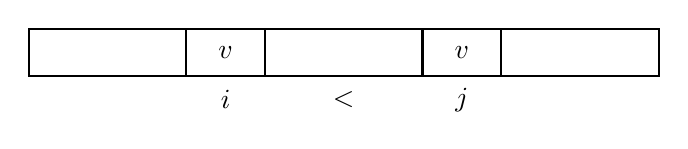
\begin{tikzpicture}[x=1cm, y=1cm]
    % Rettangolo esterno
    \draw[thick] (0,0) rectangle (8,0.6);
    
    % Linee verticali divisorie e simboli di infinito (primo blocco)
    \draw[thick] (2,0) -- (2,0.6);
    \draw[thick] (3,0) -- (3,0.6);
    \node at (2.5, 0.3) {\(v\)};
    
    % Linee verticali divisorie e simboli di infinito (secondo blocco)
    \draw[thick] (5,0) -- (5,0.6);
    \draw[thick] (6,0) -- (6,0.6);
    \node at (5.5, 0.3) {\(v\)};
    
    % Etichette inferiori
    \node at (2.5, -0.3) {\(i\)};
    \node at (4.0, -0.3) {\(<\)};
    \node at (5.5, -0.3) {\(j\)};
\end{tikzpicture}
$\quad$ Dove $i<j$ e \texttt{A[i]=A[j]}
\end{center}
\colorbox{yellow}{Osservazione}: \texttt{dup(A[p..r])=dup(A[p..q])} $\cup$ \texttt{dup(A[q+1,r])} $\cup$ \texttt{dupCross(A,p,q,r)}

\begin{info}{Idea}{}
    Per trovare i duplicati, arco-ordino l'array in modo simile al merge sort.

    Metodo \texttt{CheckCrossDup(A,p,q,r)} che prende \texttt{A[p,q],A[q+1,r]} ordinati e verifica la presenza
    di duplicati \underline{cross}, se non ce ne sono ordina \texttt{A[p..r]}.
\end{info}

Per contare i duplicati:
    \[|\left\{(i,j)|\ 1\le i<j\le n\ \wedge\ \texttt{A[i]=A[j]}\right\}|\]
\begin{verbatim}
    CountDup(A,p,r)
        if p<r
            q= (p+r)/2
            return CountDup(A,p,r)+CountDup(A,q+1,r)+CountCrossDup(A,p,q,r)
        else
            return 0;
\end{verbatim}

\section{HeapSort}
\colorbox{yellow}{Complessità}
\begin{itemize}
    \item tempo \(\Theta(n\log n)\)
    \item spazio \(\Theta(1)\)
\end{itemize}

\begin{defi}{Albero Binario Completo}{}
    \begin{enumerate}
        \item Ogni nodo non foglia ha solo due figli
        \item Ogni cammino radice-foglia ha la stessa lunghezza
    \end{enumerate}
    Quindi un albero è \textbf{completo} se ha la radice, con due figli e ognuno di essi è radice di un sotto albero completo
    della stessa altezza
\end{defi}

\colorbox{yellow}{Proposizione}: Un albero completo di altezza $h$ ha un numero di nodi $2^{n+1}-1$.

\colorbox{yellow}{Dimostrazione}: Per induzione su $h\quad n(\operatorname{T})=$ numero di nodi dell'albero $\operatorname{T}$. 
\begin{itemize}
    \item Caso base $(h=0)$: \[n(\operatorname{T})=1=2^{0+1}-1\quad\checkmark\]
    \item Passo induttivo $(n>0)$: \quad Dove $h'=h-1$, quindi:
    \[n(\operatorname{T})=n(\operatorname{T}_1)+n(\operatorname{T}_2)+1=2\left(2^{h'+1}-1\right)+1=2(2^h-1)+1=2^{h+1}-1\quad\checkmark\]
\end{itemize}

\begin{defi}{Albero binario quasi completo}{}
    Tutti i livelli sono completi tranne l'ultimo dove le foglie sono solo a sinistra.
\end{defi}

\begin{defi}{Heap}{}
    È un albero binario ordinato quasi completo implementato come array.
    
    Ci sono due tipi di \textbf{Heap}:
    \begin{itemize}
        \item \textbf{Max Heap}: Dove ogni nodo \texttt{A[i]} è $\ge$ dei suoi figli, ma $\le$ dei suoi antenati/parenti
        \item \textbf{Min Heap}
    \end{itemize}
\end{defi}

\section{QuickSort}
Complessità:
\begin{itemize}
    \item Caso peggiore: $O(n^2)$
    \item Caso medio: $O(n\log n)$
\end{itemize}
\begin{info}{Funzionamento}{}
    Come il mergeSort, applica il principio \underline{divide et impera}:

    \begin{itemize}
        \item \textbf{Partiziona}: sceglie un elemento $x$ detto \underline{Pivot} in \texttt{A[p..r]},
        adesso divide l'array in modo che ogni elemento di \texttt{A[p:q-1]} sia minore o uguale del pivot, 
        mentre ogni elemento in \texttt{A[q+1:r]} è maggiore o uguale al pivot.
        \item \textbf{Impera}: ordina \texttt{A[p:q-1]} e \texttt{A[q+1:r]} ricorsivamente
        \item \textbf{Combina}: Non fa nulla, dato che gli array sono già ordinati, non serve combinarli
    \end{itemize}
\end{info}


\section{Esercizi}
\begin{itemize}
    \item 01/10/2026
    \item 05/10/2026
\end{itemize}

\end{document}